\subsection{How Frequent is Non-Fixed-Point Behavior?}

In this section we investigate more closely the ``orbits'' and ``sliders'' initially observed by \citet{geiping2025scaling}. These are important as they appear to represent stable limiting behavior that are \textbf{not fixed points}.

We develop a heuristic algorithm to detect these behaviors, presented in \Cref{alg:orbit_slider}. We use the sequence of cosine similarities from the final recurrent layer (per token), where the output residual stream after each of 128 recurrences is compared to the final residual stream (as in \Cref{fig:fixed_point_cosine_similarities}). This is visualized in the leftmost column of \Cref{fig:orbit_algorithm_examples}. We set threshold $\tau=0.05$ and fixed-point fraction $\rho=0.9$.

Using this algorithm, we classify the limiting behavior over \emph{all} tokens in the GSM8k test set for the \raven{} and \rllama{} models. We discover that the \emph{system prompt} used before presenting the GSM8k question has a large impact on the limiting behavior types and as such we test the following prompts across both models:
\paragraph{Long Persona} This is the system prompt used by \citet{geiping2025scaling} to produce their Orbit plots:
\begin{tcolorbox}[colback=gray!10, colframe=gray!50, arc=5pt]
You are Huginn, an AI assistant who embodies careful thought and deliberation. Your responses demonstrate:

Methodical reasoning, breaking complex problems into clear steps

Mathematical and programming expertise grounded in fundamentals

The ability to acknowledge uncertainty and correct course when needed

Clear communication that illuminates rather than just informs

When engaging with questions, you first seek to understand their deeper structure before answering. Like your namesake who flew the nine worlds seeking wisdom, you explore problems from multiple angles, helping users build genuine understanding rather than providing shallow answers.
You express warmth and intellectual curiosity while maintaining professionalism. When faced with errors or confusion, you model honest reflection and careful correction. Your goal is not just to provide answers, but to help humans develop clearer, deeper thinking.
\end{tcolorbox}

\paragraph{Long Persona (Padded)} This is the same prompt as above but with all tokens replaced with the padding token: we include this to test whether the behavior arises purely due to the length of the input.

\paragraph{Short Math} This is the system prompt used by \citet{geiping2025scaling} in their GSM8k benchmark evaluation:
\begin{tcolorbox}[colback=gray!10, colframe=gray!50, arc=5pt]
You are a helpful assistant that is capable of helping users with mathematical reasoning.
\end{tcolorbox}

We present the percentage of GSM8k tokens that exhibit each classification of limiting behavior in \Cref{tab:behavior_tokens} and the percentage of GSM8k examples that exhibit each classification of limiting behavior \emph{across any of their tokens} in \Cref{tab:behavior_existence}.

These results reveal that these non-fixed-point limiting behaviors appear to be extremely rare in practice: without a system prompt (the setting used throughout this paper) only approximately 0.02\% of tokens exhibit non-fixed-point behavior. This percentage can be significantly increased with the longer system prompt, but these behaviors remain rare at 0.14\%. Curiously, the ``Persona'' system prompt used by \citet{geiping2025scaling} seems to increase the occurrence of these orbits and sliders more than a comparable prompt of padding tokens, suggesting that the effect is not purely to do with sequence length.

We highlight that these exact results need to be treated with caution: the absolute values vary significantly depending on the algorithm hyperparameters chosen, and in the absence of a good external metric we selected these hyperparameters manually via visual inspection of the trajectories and cosine similarities to ensure the results agreed with intuition. However, across different hyperparameters the results consistently showed that non-fixed-point behavior is rare and that the long persona prompt results in a greater rate of non-fixed-point behavior. We leave in-depth classification and explanation of this phenomena to future work.

\begin{algorithm}
\caption{Per-token limiting behaviour classification}\label{alg:orbit_slider}
\begin{algorithmic}[1]
\REQUIRE similarity (or norm) series $\mathbf{s} \in \mathbb{R}^{n}$ for one token
         over the last $n$ recurrent firings (final firing excluded);
         threshold $\tau$; fixed-point fraction $\rho$
\ENSURE  Label $\ell \in \{\textsc{FixedPoint},\, \textsc{Orbit},\, \textsc{Slider},\, \textsc{Unknown}\}$

\STATE \textit{--- Detrend ---}
\STATE Fit linear trend: $[\hat{a},\hat{b}] \gets \arg\min_{a,b}\sum_i (s_i - a i - b)^2$
\STATE $\tilde{\mathbf{s}} \gets \mathbf{s} - (\hat{a}\,\mathbf{t} + \hat{b})$
       \hfill $\triangleright$ $\mathbf{t} = [0, 1, \dots, n-1]^\top$

\STATE \textit{--- Spectral amplitude ---}
\STATE $\mathbf{w} \gets \tilde{\mathbf{s}} \odot \operatorname{Hann}(n)$
       \hfill $\triangleright$ reduce spectral leakage
\STATE $\mathbf{M} \gets |\operatorname{RFFT}(\mathbf{w})|_{1:}$
       \hfill $\triangleright$ discard DC bin
\STATE $k^* \gets \arg\max_k M_k$
\STATE $A \gets 4\, M_{k^*} / n$
       \hfill $\triangleright$ Hann-corrected amplitude

\STATE \textit{--- Classify (first match wins) ---}
\STATE $n_{\text{close}} \gets \#\{i : s_i \geq 1 - \tau\}$
       \hfill $\triangleright$ (or $s_i \leq \tau$ for norm)
\IF{$n_{\text{close}} \geq \rho\, n$}
    \STATE \textbf{return} $\textsc{FixedPoint}$
\ENDIF
\STATE \hfill $\triangleright$ peak-to-peak $= 2A \geq \tau$; at least 2 full cycles in window
\IF{$A \geq \tau/2$ \textbf{ and } $(k^*+1)/n \geq 2/n$}
    \STATE \textbf{return} $\textsc{Orbit}\!\left(\text{freq} = (k^*+1)/n,\; \text{amp} = A\right)$
\ENDIF
\STATE $g \gets \hat{a}$
       \hfill $\triangleright$ linear-fit slope; negate for norm series
\STATE \hfill $\triangleright$ sim increases by ${\geq}\,\tau$ over the full window
\IF{$g > \tau / n$}
    \STATE \textbf{return} $\textsc{Slider}(g)$
\ENDIF
\STATE \textbf{return} $\textsc{Unknown}$
\end{algorithmic}
\end{algorithm}

\begin{figure}
    \centering
    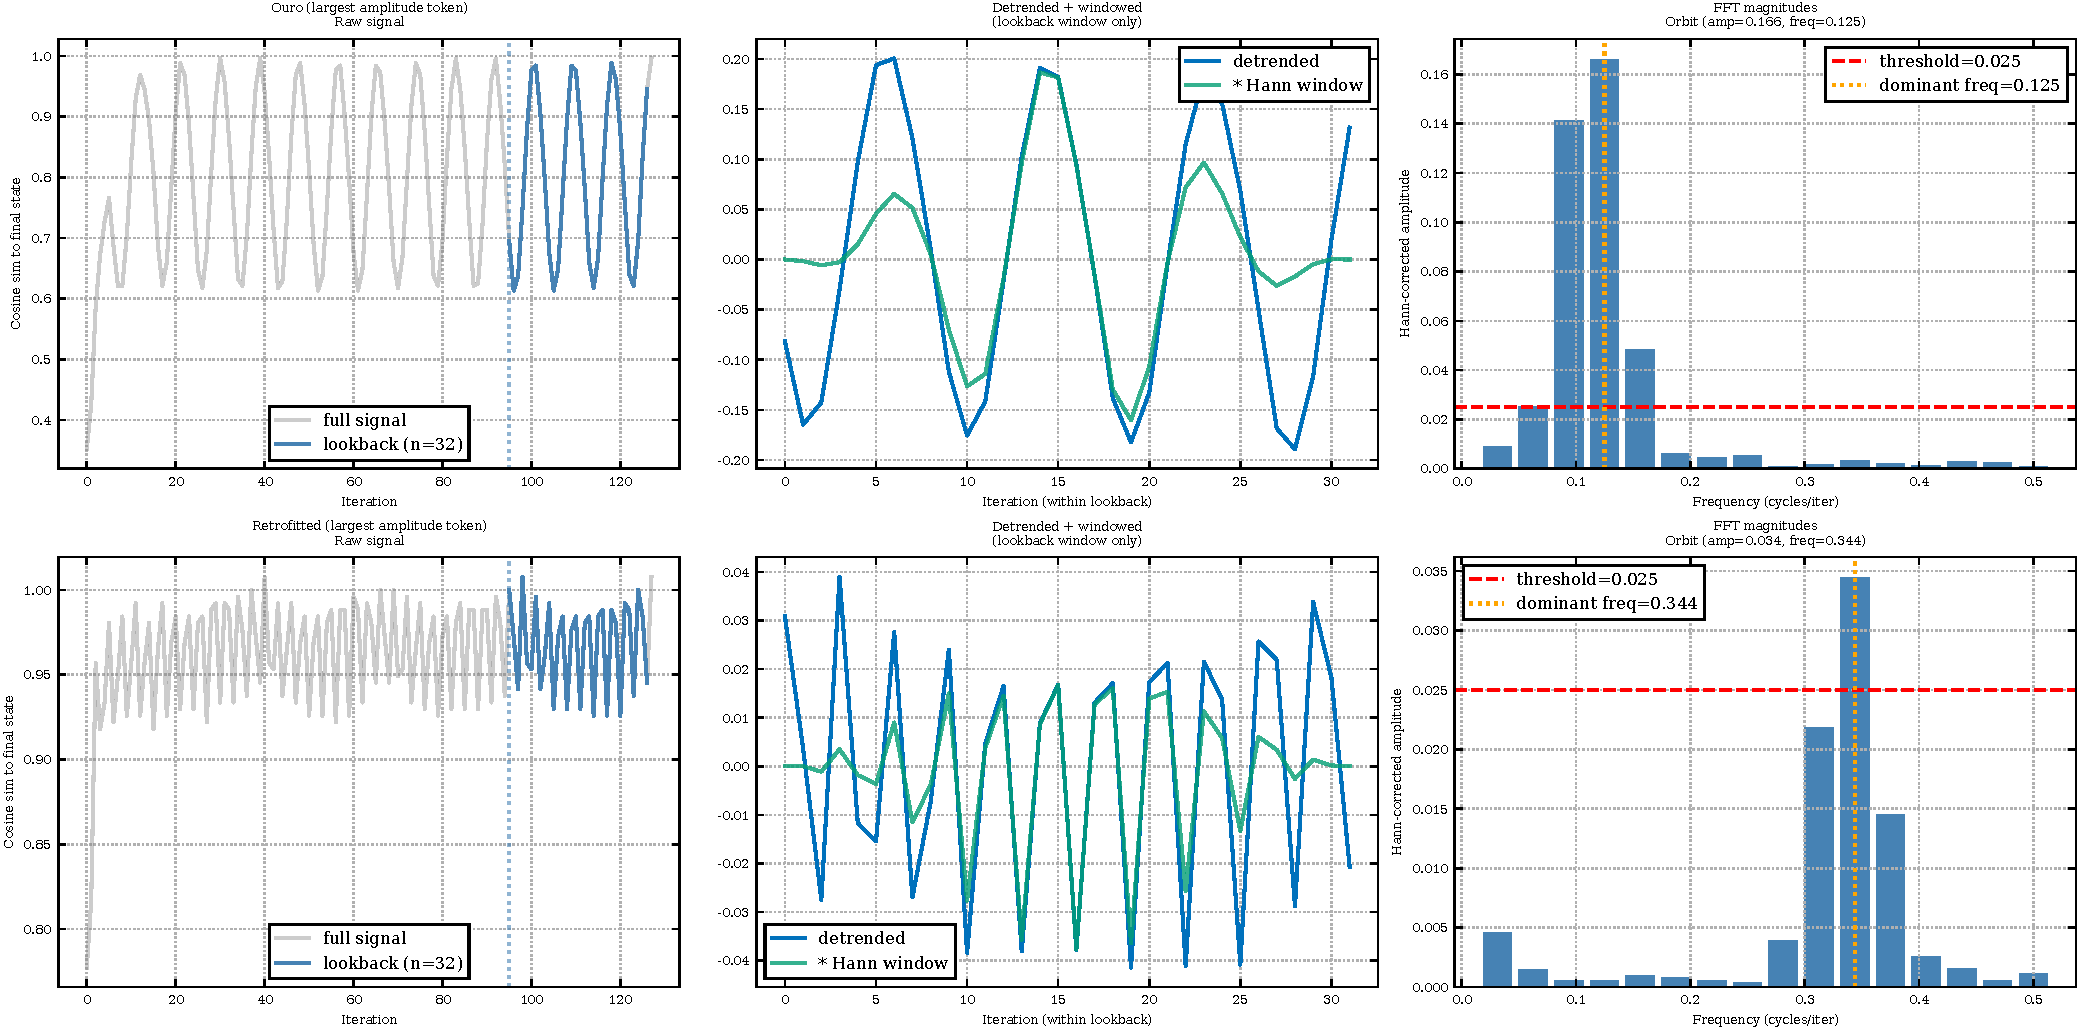
\includegraphics[width=\linewidth]{figures/orbits_sliders/orbit_algorithm_examples.pdf}
    \caption{Visualizing the component parts of the Orbit detection algorithm of \Cref{alg:orbit_slider}. The input sequence (cosine similarities for the residual streams of a given token and layer and successive recursions, as compared to their final residual stream) is visualized in the leftmost column. The center column visualizes the effect of windowing and de-trending, and the rightmost column shows the FFT magnitudes. The top row visualizes the detected Orbit with the largest amplitude for the \raven{} model (which occurs with the ``Long Persona'' prompt) and the bottom row visualizes the largest amplitude for the \rllama{} model (which occurs with no system prompt). We note the appearance of complex, multi-frequency oscillation in this latter case.}
    \label{fig:orbit_algorithm_examples}
\end{figure}

\begin{table}
\centering
\caption{Percentage of tokens exhibiting each behavior type, by model and system prompt.}
\label{tab:behavior_tokens}
\begin{tabular}{llrrrr}
\toprule
Model & System Prompt & Non-Fixed-Point \% & Orbit \% & Slider \% & Unknown \% \\
\midrule
Huginn & Long Persona & 0.14 & 0.13 & 0.00 & 0.01 \\
Huginn & Long Persona (Padded) & 0.05 & 0.02 & 0.02 & 0.01 \\
Huginn & No System Prompt & 0.02 & 0.01 & 0.01 & 0.00 \\
Huginn & Short Math & 0.01 & 0.00 & 0.00 & 0.00 \\
Retrofitted-Llama & Long Persona & 0.00 & 0.00 & 0.00 & 0.00 \\
Retrofitted-Llama & Long Persona (Padded) & 0.00 & 0.00 & 0.00 & 0.00 \\
Retrofitted-Llama & No System Prompt & 0.00 & 0.00 & 0.00 & 0.00 \\
Retrofitted-Llama & Short Math & 0.00 & 0.00 & 0.00 & 0.00 \\
\bottomrule
\end{tabular}
\end{table}

\begin{table}
\centering
\caption{Percentage of examples exhibiting each behavior type at least once on any question token, by model and system prompt.}
\label{tab:behavior_existence}
\begin{tabular}{llrrrr}
\toprule
Model & System Prompt & Non-Fixed-Point \% & Orbit \% & Slider \% & Unknown \% \\
\midrule
Huginn & Long Persona & 2.81 & 2.50 & 0.15 & 1.06 \\
Huginn & Long Persona (Padded) & 0.83 & 0.23 & 0.61 & 0.15 \\
Huginn & No System Prompt & 0.76 & 0.53 & 0.15 & 0.08 \\
Huginn & Short Math & 0.45 & 0.38 & 0.08 & 0.00 \\
Retrofitted-Llama & Long Persona & 0.00 & 0.00 & 0.00 & 0.00 \\
Retrofitted-Llama & Long Persona (Padded) & 0.00 & 0.00 & 0.00 & 0.00 \\
Retrofitted-Llama & No System Prompt & 0.08 & 0.08 & 0.00 & 0.00 \\
Retrofitted-Llama & Short Math & 0.00 & 0.00 & 0.00 & 0.00 \\
\bottomrule
\end{tabular}
\end{table}

\FloatBarrier
\subsection{Do Intermediate Layers Exhibit Non-Fixed-Point Behavior?}

\citet{geiping2025scaling} observe orbits and sliders in the latent states after each application of the entire recurrent block. Here we investigate what occurs in the latent states of the intermediate layers within the recurrent block.

We first extend Figure 16 of \citet{geiping2025scaling} (visualizing latent trajectories on a math prompt), visualizing also the trajectories of the intermediate layer residual streams: this can be found in \Cref{fig:intermediate_nfp_behavior}. This demonstrates that in this particular case, where Orbits occur, they also occur in the intermediate layers. This implies -- viewed in realized depth -- latent trajectories exhibiting multi-scale cyclic behavior.

We investigate this across all GSM8k test examples in \Cref{fig:nfp_behavior_conditional_probability} by plotting the conditional probability of observing each behavior on a given token for any layer, given an observation of observing another behavior on that same token. We discover that orbits and sliders do not co-occur across looped layers, but that orbits and sliders both frequently co-occur with fixed point behavior. ``Unknown'' behavior often co-occurs with orbits, which we suggest may be due to mis-classification of the behavior algorithm.

\begin{figure}[ht]
    \centering
    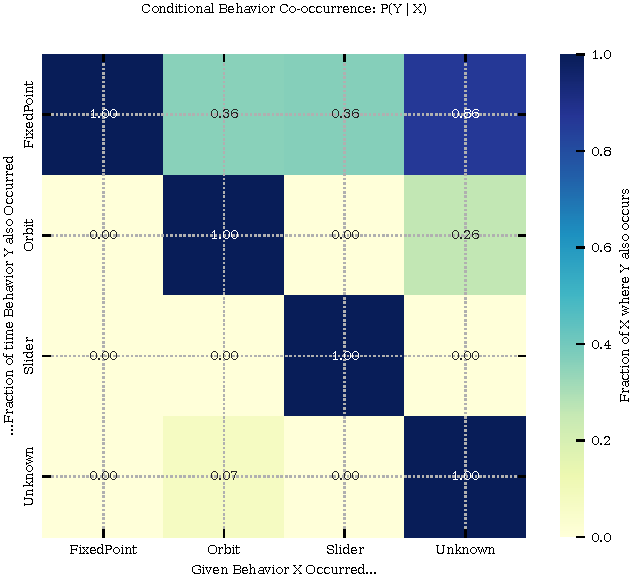
\includegraphics[width=0.6\linewidth]{figures/orbits_sliders/behavior_cooccurrence_heatmap.pdf}
    \caption{Conditional probabilities of co-occurrence for the different limiting behaviors.}
    \label{fig:nfp_behavior_conditional_probability}
\end{figure}

\begin{figure}
    \centering
    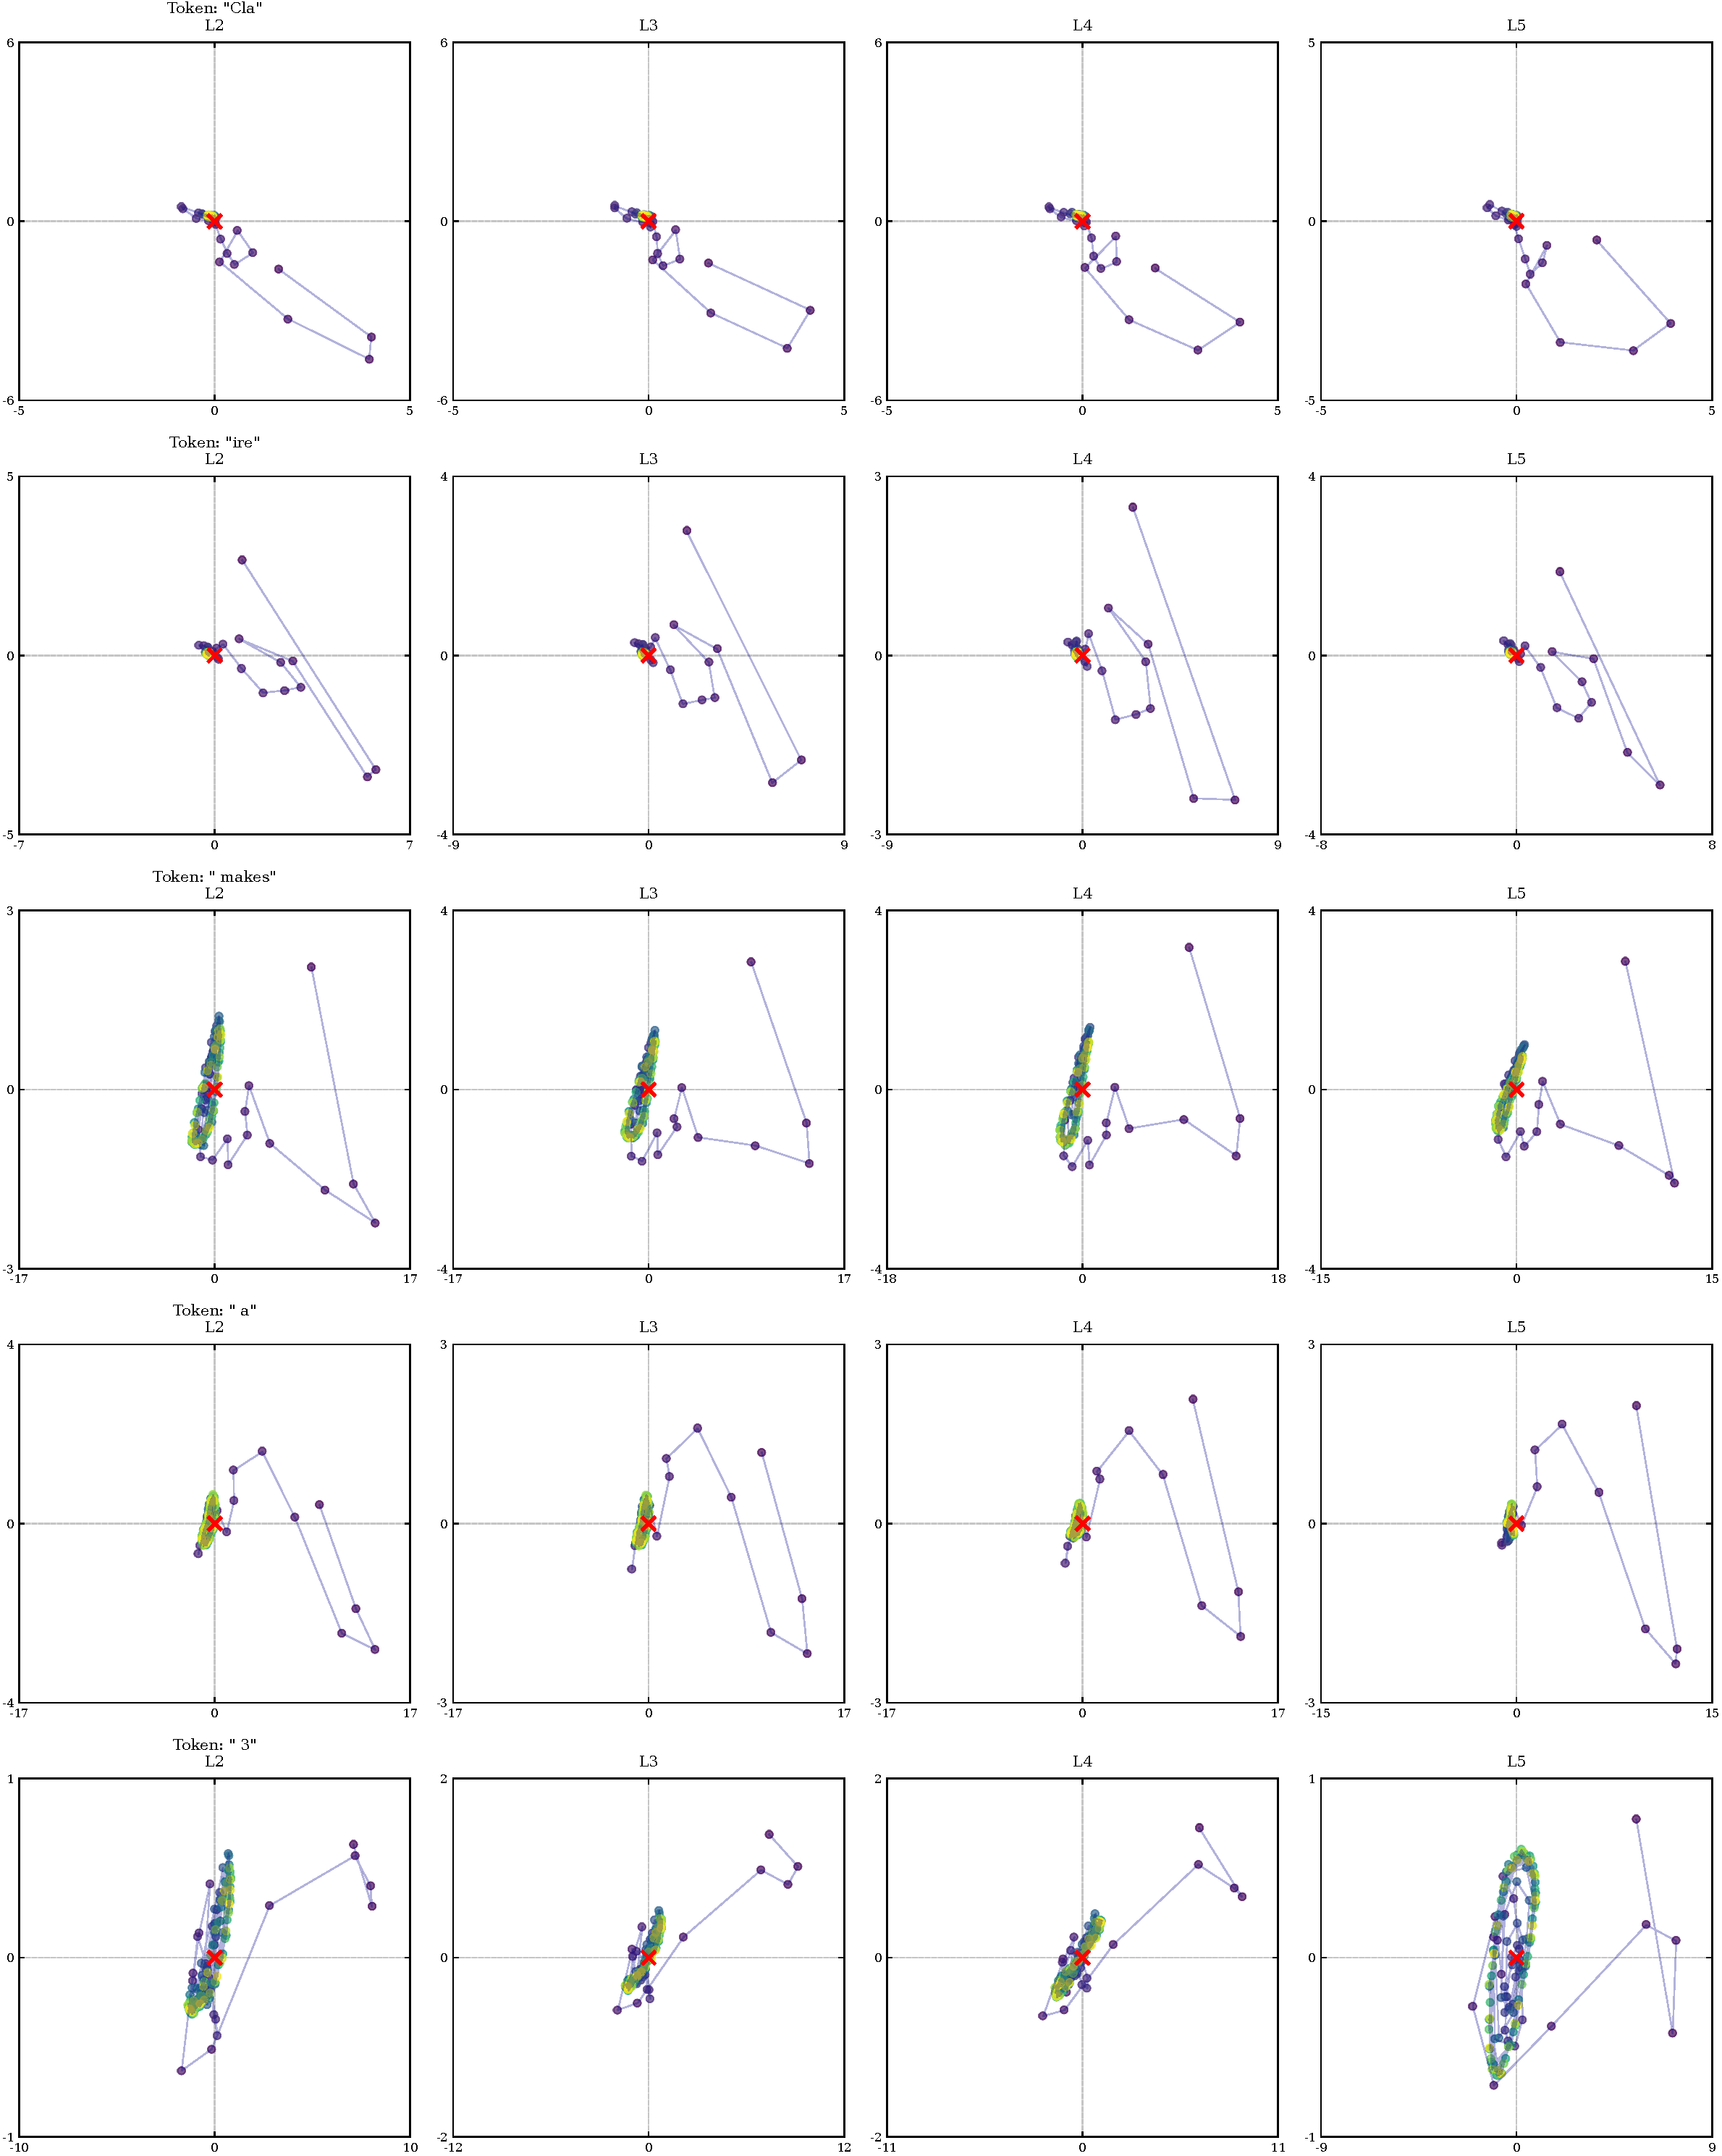
\includegraphics[width=\linewidth]{figures/orbits_sliders/pca_intermediate.pdf}
    \caption{PCA trajectories in the intermediate layers of \raven{}: this reproduces the leftmost column of Fig. 16 in \citet{geiping2025scaling} (the first two principal components) and additionally plots the latent trajectories for the intermediate layers in the recurrent block.}
    \label{fig:intermediate_nfp_behavior}
\end{figure}

\FloatBarrier
\subsection{How Does Non-Fixed-Point Behavior Impact Stages of Inference?}

To complete the link between non-fixed-point behavior and our work we additionally investigate how this behavior impacts the observed stages of inference.

To attempt to isolate the ``worst case'' scenario for stages of inference stability, we plot stages of inference for the GSM8k test prompt that exhibits the greatest orbit amplitude. We first plot in realized depth the extended stages of inference metrics used throughout the paper, see \Cref{fig:orbits_sliders_huginn_stability_in_recurrence}. This demonstrates that sink rates show some variability with the orbiting behavior, but the other metrics remain broadly consistent. We plot also the same metrics in block depth (showing only the final 64 loops) in \Cref{fig:orbits_sliders_huginn_stability_in_depth}: this demonstrates clearly that the stages of inference remain very consistent despite the orbiting behavior.

\begin{figure}[ht]
    \centering
    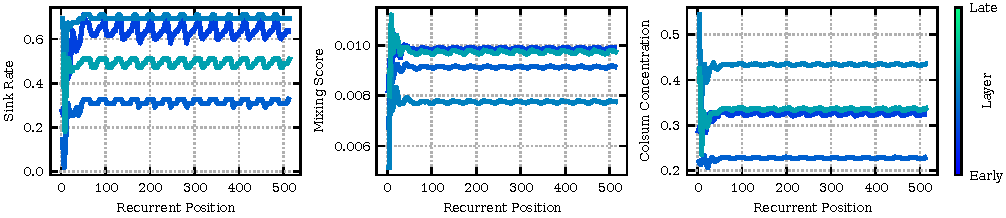
\includegraphics[width=\linewidth]{figures/orbits_sliders/huginn_stability_in_recurrence.pdf}
    \caption{Stages of inference metrics (sink rate, mixing score and colsum concentration) for \raven{} across 128 recurrences, for the GSM8k test prompt that exhibited the largest orbit amplitude. Visualized in realized depth.}
    \label{fig:orbits_sliders_huginn_stability_in_recurrence}
\end{figure}

\begin{figure}[ht]
    \centering
    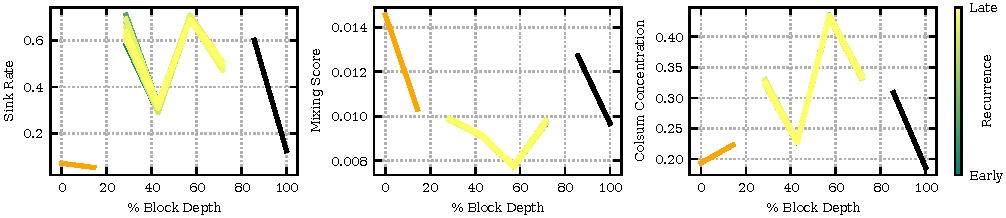
\includegraphics[width=\linewidth]{figures/orbits_sliders/huginn_stability_in_percentage_depth.pdf}
    \caption{Stages of inference metrics (sink rate, mixing score and colsum concentration) for \raven{} across 128 recurrences, for the GSM8k test prompt that exhibited the largest orbit amplitude: only the final 64 recurrences are visualized, to isolate the impact of the orbit. Visualized in percentage block depth.}
    \label{fig:orbits_sliders_huginn_stability_in_depth}
\end{figure}

We plot the same for the largest amplitude orbit on the \rllama{} model in \Cref{fig:orbits_sliders_llama_stability_in_depth}, demonstrating that the same behavior holds.

\begin{figure}[ht]
    \centering
    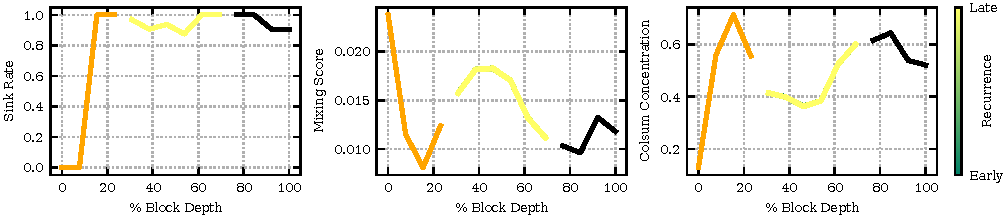
\includegraphics[width=\linewidth]{figures/orbits_sliders/stability_in_percentage_depth_llama.pdf}
    \caption{Stages of inference metrics (sink rate, mixing score and colsum concentration) for \rllama{} across 128 recurrences, for the GSM8k test prompt that exhibited the largest orbit amplitude: only the final 64 recurrences are visualized, to isolate the impact of the orbit. Visualized in percentage block depth.}
    \label{fig:orbits_sliders_llama_stability_in_depth}
\end{figure}